\documentclass[draft, 12pt]{article}
\usepackage[english]{babel}
\usepackage[final]{graphicx}
\usepackage{multirow}
\usepackage{color}
\graphicspath{ {figures/} }
\DeclareGraphicsExtensions{.png}

\newcommand{\cc}[1]{\textcolor{red}{#1}}

\title{Seismic parameter estimation and the Canadian crust}
\author{Ben Postlethwaite}

%% ------------------------------------------------------------------------ %%
\begin{document}

\begin{abstract}

\end{abstract}

%% -----------------------------------------------%%
\section{Introduction}

%% Seismic studies of the Canadian continental crust predominately analyze specific geological features or regions rather than taking a comprehensive and comparative inter-regional analysis. The primary reason for this is the poor resolution afforded by the seismic networks currently and historically deployed across Canada. The Canadian continental landmass is composed of at least fifteen large geological provinces as recognized by the Geological Survey of Canada (GSC). Each of these regions is itself complex and heterogeneous and often larger than most European nations. On top of this there is poor seismic coverage, roughly one seismic station per 25,000 $km^2$. Many of these stations are clustered near areas of geologic interest such as the Cascadia Subduction zone or population and research centres such as Southern Ontario or areas of significant resource interest like the diamondiferous Great Slave Lake area. This leaves vast areas of the Canadian landmass completely unsampled. Despite these limitations, a low resolution comprehensive and comparative study is still feasible for some of the geological regions comprising the Canadian continental crust. Direct comparison between the bulk average seismic properties of geological regions and between aggregated regions and global averages provide some new insight into the crustal composition of the Canadian landmass. The accumulated dataset also affords investigations into variations of bulk crustal parameters such as Poisson's Ratio and crustal thickness with age and tectonic environment as well as some basic statistical data on interesting crustal features.

%% This paper presents a comparative tour through the dataset accumulated from processing more than a decade worth of data from all available Canadian seismic stations. It begins with a discussion of the raw data itself followed by a review of the receiver function method and a more detailed explanation of the inversion algorithms used to produce the dataset. Three previous publications utilizing similar processing schemes provide unique subsets of data to compare with the values computed in this survey for quality assurance. ...


\subsection{Geological and tectonic summary}
\begin{itemize}

\item Large scale overview/summary of regions under study
\item Justification for selecting these regions?

\end{itemize}

\subsection{Previous geophysical studies}
\begin{itemize}

\item Lithoprobe and attendent papers
\item Teleseismic studies

\end{itemize}
%% -----------------------------------------------%%
\section{Data and methods}
Our analysis of bulk Canadian continental crust is based on estimates of crustal properties that can be accessed via seismic techniques, namely seismic wave velocities (or velocity ratio) and crustal thickness. This study draws on three sources for these crustal properties. The first and primary source is teleseismic receiver function (hereafter RF) analysis. The remaining two datasets are Crust 1.0, a widely published statistical average of similar regions with a global two degree resolution, and a compilation of pre-processed active source data (Mooney, 2012). Both Crust 1.0 and the active source compilation are used to qualify and compare with the primary dataset.

\subsection{Teleseismic Data Set}
The primary data utilized in this study are computed from teleseismic {\it P} wave seismograms originating from more than 700 earthquake sources. These earthquakes occurred between 2000 and 2012 and were recorded on subsets of 343 broadband seismic stations distributed across Canada. Seismic stations are selected from all available regional and national networks including CNSN, POLARIS, FedNor and Chasme. Seismograms are included for analysis if they fall within a 30 to 100$^\circ$ epicentral distance window. Quality control is performed by admitting only those seismograms with sufficiently high signal to noise ratios to permit visual observation of the dominant {\it P} wave energy and with sufficiently impulsive first arrivals to allow arrival onsets to be accurately measured. After selection and filtering more than 80,000 events are available for further processing.

The first stage of processing requires the transformation of teleseismic data into receiver functions. In general terms, this transformation involves deconvolving an approximation of the earthquake source from horizontal recordings of ground motion [Langston, 1979]. The resulting waveforms contain discrete pulses corresponding to {\it S} waves scattered from subsurface discontinuities including the base of the crust, or Moho. Confident identification of these peaks is required to estimate crustal parameters, and improved results can be obtained by transforming the displacement seismogram into their {\it P} and {\it S} contributions based on a 1-D model of propagation. This procedure is accomplished by first rotating the N and E coordinates into radial and transverse directions and then performing a wave field decomposition using the radial and vertical channels [Kennet, 1991]. The direct {\it P} arrival of the signal on the resulting {\it P} wave component is used as an approximation to the source function as {\it P} component impulse response for teleseismic P approximates a delta function. This windowed source estimate is deconvolved from the {\it S} wave component computed from the wave field decomposition.

We employ an $L_2$, multichannel, frequency domain approach to perform the deconvolution that has the advantage of computational efficiency and does not require {\it a priori} assumptions concerning the noise levels in the data. More specifically, we employ a simultaneous deconvolution of $N$ seismograms sharing a similar slowness to compute a single impulse response or receiver function $r(t)$.

% Deconvolution equations
\begin{equation}
  r(t) = {\cal F}^{-1} \left[ G(\omega) \right] = {\cal F}^{-1}
 \left[ \frac {\sum_n^N S_n(\omega)P_n^*(\omega)} {\sum_n^N P_n(\omega)P_n^*(\omega) + \delta} \right ],
\end{equation}

\noindent where $F^{-1}$ is the inverse Fourier transform, $S_n$ represents the $n^{th}$ {\it S} wave seismogram, $P_n$ is the corresponding windowed {\it P} wave seismogram, $^*$ denotes complex conjugation and $\delta$ is the regularization parameter controlling the trade off between model smoothness and data misfit. The parameter $\delta$ which is chosen programatically by minimizing the general cross validation function $GCV(\delta)$ is given by

\begin{equation}
  GCV(\delta) = \frac {\sum_n^N\sum_m^M \left( S_n(\omega_m) - P_n(\omega_m)G(\omega_m) \right)^2 }
                      { \left( NM - \sum_m^M X(\omega_m) \right)^2 },
\end{equation}

\noindent where

\begin{equation}
  X(\omega_m) = \frac {\sum_n^N P_n(\omega_m)P_n^*(\omega_m)} {\sum_n^N P_n(\omega_m)P_n^*(\omega_m) + \delta},
\end{equation}

\noindent and $\omega$ is the frequency bin in the discrete Fourier transform. All resulting receiver functions, $r(t)$, are filtered between 0.04Hz and 3.0Hz.

\subsection{Vp/Vs method} \label{section:VpVsMethod}

\begin{figure}
  \centering
    \includegraphics[width=\textwidth]{reflectedPhases}
  \caption{Schematic diagram illustrating geometry of phases for the velocity contrast representing the Moho}
  \label{fig:reflectedPhases}
\end{figure}


A well tested and widely published method for extracting the ratio of {\it P} velocity $V_P$ to {\it S} velocity $V_S$, herafter referred to as $R$, and crustal thickness (or depth to Moho) $H$, is outlined by Zhu and Kanamori [2000], hereafter ZK. This method exploits the dependence of these parameters to the differential arrival times between the {\it S} wave reflected phases $Ps$, $PpPs$, $PsPs$, $PpSs$ and $PsSs$ and the direct {\it P} wave arrival $Pp$ (Fig \ref{fig:reflectedPhases}). Note that $PsPs$ and $PpSs$ are kinematic analogues, such that the energy for these two phases arrive simultaneously for a 1-D model. For a range of slowness values, $p$, the differential arrival times, $t(p)$, trace moveout curves for each phase arrival given by

% Travel time equations
\begin{equation} \label{eq:tps}
t_{Ps}(p_n) = \frac{H}{V_P} \left[ \sqrt{ R^2 - V_P^2p_n^2} - \sqrt{1 - V_P^2p_n^2} \right]
\end{equation}

\begin{equation}
t_{Pps}(p_n) = \frac{H}{V_P} \left[ \sqrt{ R^2 - V_P^2p_n^2} + \sqrt{1 - V_P^2p_n^2} \right]
\end{equation}

\begin{equation}
t_{Pss}(p_n)= \frac{2H}{V_P} \sqrt{ R^2 - V_P^2p_n^2}
\end{equation}

\noindent where $p_n$ is the slowness for the $n^{th}$ receiver function. Since strong reflected phases occur at sharp velocity contrasts, the Moho, the boundary targeted by ZK, tends to be well represented on most RF's.

The travel time equations, as employed by ZK, assume a value for crustal {\it P} wave velocity, $V_P$, that in practice will trade-off to some degree with crustal thickness $H$. In our implementation of the ZK approach, each station is assigned a $V_P$ value corresponding to the Crust 1.0 value for the corrisponding $2^\circ$ containing cell. In the specific cases where data are being compared to previously published results for quality control, $V_P$  values are chosen to match the values in the published study.

RFs are stacked along trial moveout curves for a range of candidate models of $R$ and $H$ to generate a fitness function $s(H,R)$.  Within the stacking procedure, each phase is assigned a weight to account for the expected relative amplitudes of the phases for typical velocity contrasts, with the direct conversion $Ps$ usually characterized by the highest quality signal followed by $PpPs$ and $PpSs$. We chose weights of $w1 = 0.5$, $w2 = 0.3$ , $w3 = -0.2$ for the $Ps$, $PpPs$ and $PpSs$ phases, respectively. A negative weight for the combined $PpSs$ and $PsPs$ phases is required as the polarity of the signal is reversed. Semblance weighting [Eaton, 2006] is employed to reduce the effect of spurious large amplitude noise in the data. The semblance function assigns a weight between zero (incoherent noise) and one (coherent signal). The stacking function is therefore defined as

\begin{equation}  \label{eq:stack}
s(H,R) = \sum_{m=1}^{3} S_m \sum_{n=1}^N w_mr_n(t_m)
\end{equation}

\noindent where

\begin{equation}
S_m(H,R) = \frac {\left[ \sum_{n=1}^N r_n(t_m) \right]^2}
                 { \sum_{n=1}^N r_n^2(t_m) }
\end{equation}

\noindent is the semblance weight for the $m^{th}$ phase, time $t_m$ is calculated from the corresponding travel time function for a given $H$, $R$ pair as a function of slowness $p_n$ and $N$ is the total number of receiver functions. Multiplying by the semblance weighting sharpens the stacked image, $s(H,R)$, and results in better resolution when discriminating between different models. The function $s(H,R)$ can be thought of as a transformation that maps times of the $Ps$, $PpPs$ and $PpSs+PsPs$ phases into $R$ and $H$ space as positive bands, via Eq. \ref{eq:stack}. Constructive interference where these bands intersect produce a maximum in the stacking function. The model, $R$ and $H$, that produces this maximum provides the best estimate for the bulk crustal parameters for a given seismic station.

%% [[\subsection{Full Parameter Method}]]
A limitation of the ZK approach is the requirement of an initial $V_P$ estimate. In principal we may compute the stacking function Eq. \ref{eq:stack}, as a function of all three seismic parameters, $s(H,R,V_P)$. Taking advantage of modern multi-core systems with reasonable quantities of data (fifty to a few hundred RFs) and a moderate search space ($n^3$ parameter candidates where $n \approx 150$) the computational time makes this method easily scalable to hundreds of stations. This ``fullgrid'' approach is analyzed to determine the viability of recovering $V_P$.

The trade-off between $V_P$ and $H$ (and other parameter combinations) and error resulting from data quality are quantified for both the full parameter search and ZK methods by bootstrap resampling [Efron and Tibshirani, 1986]. An estimate for the error is calculated in a bootstrap resampling approach by taking the standard deviation of 1024 parameter estimates each produced with randomly selected RFs, with replacement.

\subsection{Additional data}

We supplement receiver function estimates of crustal properties with data from controlled source experiments collected and compiled from GSC (Geological Survey of Canada) references by Walter Mooney (personal communication, 2012). The active source data provide $V_P$ and a few $V_S$ estimates for hundreds of locations across Canada, many along transects that cross major geological boundaries, faults and discontinuities. Some of these data are located within reasonable ($<$100 km) proximity to seismic stations used in this study and can be used to compare with the $V_P$ and $V_S$ estimates resulting from the RF full gridsearch.

The Crust 1.0 model [Laske et. al., 2013] employs many of these same active source data to provide regular, complete coverage across all of Canada. The model includes estimates of $V_P$ and $V_S$ information with depth at $1^\circ$ resolution in latitude and longitude. In addition to employing local active source data, Crust 1.0 is also constrained by statistically aggregated data from geographically distant but geologically similar regions. It therefore affords a somewhat independent dataset suited for comparison with the crustal estimates calculated in this study.

%% -----------------------------------------------%%
\section{Results}

\subsection{Comparisons}

Three published studies have provided parameter estimates for $R$ and $H$ for subsets of the seismic stations considered here. The most recent study [Thompson et. al., 2010] focused on the northern Canadian Shield and employs both the linear stacking approach used by ZK as well as a phase weighted method. A 2007 study of the Superior Province [Darbyshire et. al, 2007] and a study of the Grenville Orogen [Eaton et. al., 2006] utilize the ZK + semblance approach outlined in section \ref{section:VpVsMethod}.  Comparisons between crustal estimates of $R$ for particular seismic stations are made for those values with corresponding standard errors of less than $\pm$0.06. This error threshold is chosen empirically as that which best partitions those receiver function stacks with visually recognizable energy along phase moveout curves from those where lack of data or poor quality make these moveout curves difficult to distinguish. For each study under comparison, data are reprocessed using the $V_P$ chosen by the study authors. For the 2006 and 2007 studies the ZK + semblance method is used whereas for the Thompson et. al study the linear stacking ZK approach is employed. Both correlation coefficient and mean difference are provided in (Table \ref{table:comparison}) as measures of similarity.

\begin{table}
  \begin{tabular}{ l l l l l l l}
    \cline{4-7}
    & & \multicolumn{2}{ c }{Correlation Coeff.} & \multicolumn{2}{ c }{RMS difference} \\
    \hline
    Study Authors             & Region         & Num. of Stns &  $H$ & $R$  &$H$(km)& $R$ \\
    \hline
    Thompson et. al. (2010)   & Northern Canadian Sheild & 29 & 0.97 & 0.70 & 0.78 & 0.017 \\
    Darbyshire et. al. (2007) & Superior Province        & 10 & 0.95 & 0.43 & 1.71 & 0.037 \\
    Eaton et. al. (2006)      & Grenville Orogen         & 26 & 0.90 & 0.61 & 1.03 & 0.033 \\
    \hline
  \end{tabular}
  \caption{Comparison of $R$ and $H$ estimates with three published studies}
\label{table:comparison}

\end{table}

All three studies reported $H$ estimates that correlate strongly with the crustal thickness parameters computed here. The data from the northern Canadian Shield shows strong correlation in both $H$ and $R$. The lower correlation observed in estimates of $R$ than $H$ is not unexpected as the range of $R$ is relatively narrow and small changes ($\approx 2\%$) are physically meaningful. A corollary of this is greater sensitivity of $R$ to differences in procedure such as the choice of deconvolution algorithm and selection and scaling of data. The results from Thompson et. al. [2010] also corrispond most closely to the parameter estimates computed here, with the mean difference for both parameters being less than half of the averaged bootstrap error computed in this study. Results published by {\it Eaton et. al.} [2006] show reasonable correlations in both $R$ and $H$ and a mean difference for both parameters that is roughly equal to the averaged uncertainty in the data. Parameter estimates from the Superior Province [Darbyshire et. al., 2007] show the lowest correlation in $R$ as well as the highest mean difference in both parameters. These differences are well over the averaged computed error, and can not be easily explained by deviation related to noise in the data.

\subsection{Full Grid Search Analysis}

We now proceed to compare our results computed using the ZK approach with those from the full grid search (Table \ref{table:ZKvsFG}). We note that the velocity ratio $R$ has a correlation between the two datasets of 0.76 whereas $H$ has a correlation of 0.51. The low correlation between crustal thickness estimates can be explained by the strong tradeoff between $H$ and $V_P$ through the quantity

$$\frac{t_{Pps}-t_{Ps}}{2}=\frac{t_{Pss}}{2} - t_{Ps}= \frac{H}{V_P}\sqrt{1-p^2V^2_P)}.$$

\noindent As a consequence, contours of the misfit surface $s(H,R,V_P)$ are highly extended along the kinematic curve in the $H$ - $V_P$ space (Figure \ref{fig:HVp_ULM}). This trade-off contributes to the low correlation in $H$ between the two methods. Higher correlation in this quantity can be restored by dividing out $V_P$ from $H$. The trade-off between the other parameters is lower as there is greater dependence between them such that a small change in one necessitates a large change in an other to maintain travel-time equality, which has the result of a well defined misfit surface (Figures \ref{fig:HR_ULM}-\ref{fig:RVp_ULM}.

For all but the cleanest stations, the trade-off between $H$ and $V_P$ renders recovery of $V_P$ unfeasible using the full grid approach. A comparison between two stations, ULM, the station with the highest quality RFs, and DORN, a station exhibiting less resolution in the reflected phases, illustrates this difficulty. RFs are arranged vertically, ordered by increasing slowness, and shown in figures \ref{fig:RF_ULM} and \ref{fig:RF_DORN}. Cross sections of $s(H,R,V_P)$ through each coordinate plane are displayed for ULM and DORN in figures \ref{fig:HR_ULM}-\ref{fig:HVp_ULM}) and figures \ref{fig:HR_DORN}-\ref{fig:HVp_DORN}. The lower resolution apparent in the $H$ - $V_P$ cross section for DORN translates into a bootstrap error of $V_P \pm 0.64 {\rm km/s}$. Station ULM, with cleaner data, has less trade-off between $H$ and $V_P$ as indicated by the corresponding cross section and the lower bootstrap error of $V_P \pm 0.16 {\rm km/s}$.

Active source experiments located near broadband seismic stations provide independent crustal thickness and {\it P} wave velocity estimates to test against data derived from the full parameter search method. We select stations with low error in $V_P$ and active source experiment locations within a 100 km radius. If several active source experiments are located within this radius, estimates are averaged. Four stations (ARVN, TYNO, ULM and WHY) meet these criteria and the parameter estimates are presented in figure \ref{fig:activeVp}-\ref{fig:activeH}. Estimates computed from the full grid approach are roughly 0.25 km/s higher than the active source data. This difference is consistent across all four stations and is exemplified by a 99\% correlation, suggesting possible bias. However, the limited number of data means this bias is poorly constrained.

There is less correlation between the crustal thickness data, though this is largely attributed to an approximate 10 km difference between the ARVN estimates. The reason for this discrepancy is unknown though both the ZK method and and a published study [Thompson et. al., 2010] provide an estimate of near 41 km for ARVN, much nearer the full grid value of 42 km. Despite lower correlation the apparent bias towards higher values computed from teleseismic data is also maintained for $H$. A positive bias in one parameter will tend to bias the other, owing to the relationship between thickness, velocity and times of a scattered phase. For a constant $t_{ps}$ one may compute how much $H$ must change for a 0.25 km/s bias in $V_P$ [Zhu and Kanamori, 2000]. Using an average of the parameter estimates from the two cleanest stations, ULM and WHY, $\delta H$ will be 1.3 km, this fits well with the actual bias in the values.

[[ SOURCES REGARDING BIAS ]] [[ WHAT DOES THIS MEAN, IS VP USABLE FOR THE HIGHEST QUALITY STATIONS?]]


\begin{table}
  \begin{tabular}{ l l }
    \hline
    Parameter & correlation coeff \\
    \hline
    $R$ (km) &  0.76 \\
    $H$      &  0.51 \\
    $H/V_P$  &  0.96 \\
    \hline
  \end{tabular}
  \caption{Correlation between parameters computed from ZK + semblance and full parameter search methods}
\label{table:ZKvsFG}

\end{table}


\begin{figure}
  \centering
  \includegraphics[width=\textwidth]{RF_ULM}
  \caption{}
  \label{fig:RF_ULM}
\end{figure}

\begin{figure}
  \centering
  \includegraphics[width=\textwidth]{stackHR_ULM}
  \caption{}
  \label{fig:HR_ULM}
\end{figure}

\begin{figure}
  \centering
  \includegraphics[width=\textwidth]{stackRVp_ULM}
  \caption{}
  \label{fig:RVp_ULM}
\end{figure}

\begin{figure}
  \centering
  \includegraphics[width=\textwidth]{stackHVp_ULM}
  \caption{}
  \label{fig:HVp_ULM}
\end{figure}

\begin{figure}
  \centering
  \includegraphics[width=\textwidth]{RF_DORN}
  \caption{}
  \label{fig:RF_DORN}
\end{figure}


\begin{figure}
  \centering
  \includegraphics[width=\textwidth]{stackHR_DORN}
  \caption{}
  \label{fig:HR_DORN}
\end{figure}

\begin{figure}
  \centering
  \includegraphics[width=\textwidth]{stackRVp_DORN}
  \caption{}
  \label{fig:RVp_DORN}
\end{figure}

\begin{figure}
  \centering
  \includegraphics[width=\textwidth]{stackHVp_DORN}
  \caption{}
  \label{fig:HVp_DORN}
\end{figure}

\begin{figure}
  \centering
  \includegraphics[width=\textwidth]{activeSourceCompVp}
  \caption{\it{P} wave velocity estimates computed from the full parameter search method compared to active source data and values from Crust 1.0}
  \label{fig:activeVp}
\end{figure}

\begin{figure}
  \centering
  \includegraphics[width=\textwidth]{activeSourceCompH}
  \caption{Crustal thickness estimates computed from the full parameter search method compared to active source data and values from Crust 1.0}
  \label{fig:activeH}
\end{figure}


\subsection{Crustal Discontinuities}

\begin{figure}
  \centering
  \includegraphics[width=\textwidth]{conradPCA}
  \caption{The SVD singular vectors (principal components) of the station depth profile matrix. Each principal component represents a mode that captures some part of the total variance in the dataset. Vertical lines are the axis each profile and vector is normalized about. A grey horizontal window highlights a region of low energy.}
  \label{fig:conradPCA}
\end{figure}

We now consider the average crustal structure across Canada. We produce a depth profile for each station by stacking receiver functions along traveltime curves corresponding to a range of values in $H$ (0 to 50 km in increments of 100 metres) using the estimates for $R$ computed via the ZK + semblance method. The resulting profiles contain energy at depths corresponding to major velocity discontinuities. By assembling all depth profiles into a matrix, we may decompose the data via SVD into their principal components. Figure \ref{fig:conradPCA} contains the first five singular vectors or modes normalized to unit magnitude that account for 78\% of the variance in the profiles. Higher modes correspond to diminishing contributions to total variance. Each vector is normalized to unit magnitude. The first mode (blue) is effectively the average depth profile across all stations and captures 50\% of the variance in the dataset. It features a maximum near 38.7 km that may be taken as an average Moho depth. The second and third modes are dominated by a high amplitude shallow structures (e.g. sedimentary layers) within the top 10 km and Moho variability between 30 and 46 km . The fourth and fifth modes account for a combined 11\% of the variance in the dataset, contain energy at upper-mid crustal depths in the 10 km to 20 km range. All 5 modes display markedly lower energy within a depth window roughly between 20 km and 30 km.

\subsection{Regional Bulk Crustal Parameters}

We proceed to consider crustal thickness $H$ and velocity ratio, $R$, estimates for stations with assigned $R$ bootstrap errors below $\pm 0.06$ in a geographic context (figure \ref{map:stationMap}). To compensate for the uneven distribution of seismic stations, weights are applied to both $R$ and $H$ estimates before averaging over a given region. Weights are calculated by projecting station locations onto a 2D plane using the Albers equal-area conic projection. A Voronoi diagram is then computed using all projected station locations. The ratio between the Voronoi cell surface encompassing each station and the total area of the convex hull bounding region is employed as that station's weight.

Table \ref{table:regionParameters} displays the results of our regionalization in $R$ and $H$. The weighted average crustal thickness for all stations (Canada) is 37 km, about two kilometres thinner than the average for the Canadian Shield. Crust 1.0 provides a slightly thicker crustal average for Canada (38.1 km) and a slightly thinner average for the Shield (38.3 km). The Slave Province averages are similar to those for the Churchill province with a crustal thickness and seismic velocity ratio comparable to Crust 1.0. Moving south and east from the Churchill Province through the Superior Province into the Grenville Province, we note an increase in the ZK + semblance $R$ values as well as crustal thickness $H$, figures \ref{map:Hmap}-\ref{map:Rmap}. The weighted $R$ average is 1.73 in the Churchill Province increasing slightly to 1.74 in the Superior and jumping to 1.78 in the Grenville. In a similar fashion, the weighted average of $H$ increases from 38.9 km in the Churchill Province  to 39.7 in the Superior Province and 41.7 km in the Grenville Province. The southeastern trend towards increasing values is also expressed in weighted averaged active source $V_P$ data as well as as the Crust 1.0 $V_P$ data.  The Crust 1.0 model is characterized by slightly thinner crust though the southward thickening trend is noticeable. The trend in the seismic velocity ratio is not, however, as apparent.


\begin{table}
  \begin{tabular}{ l l l l l l l }
    \cline{2-7}
    & \multicolumn{2}{ c }{ZK + semblance} & \multicolumn{3}{ c }{Crust 1.0} & \multicolumn{1}{ c }{Active Source} \\
    \hline
    Region  & $H [km]$& $R$ &$H [km]$& $R$  &$V_P [km/s]$&$V_P [km/s]$ \\
    \hline
    Canada    & 37.0 & 1.75 & 38.1   & 1.74 &   6.41     & 6.33\\
    Shield    & 39.2 & 1.74 & 38.3   & 1.74 &   6.47     & 6.42\\
    Slave     & 38.2 & 1.74 & 38.0   & 1.73 &   6.47     & 6.44\\
    Churchill & 38.9 & 1.73 & 37.9   & 1.74 &   6.46     & 6.39\\
    Superior  & 39.7 & 1.74 & 38.9   & 1.74 &   6.49     & 6.44\\
    Grenville & 41.7 & 1.78 & 39.7   & 1.74 &   6.50     & 6.48\\
    \hline
  \end{tabular}
  \caption{Comparison of $R$ and $H$ estimates with three published studies}
\label{table:regionParameters}

\end{table}


\begin{figure}
  \centering
  \includegraphics[width=\textwidth]{stationMap}
  \caption{}
  \label{map:stationMap}
\end{figure}

\begin{figure}
  \centering
  \includegraphics[width=\textwidth]{Hmap}
  \caption{}
  \label{map:Hmap}
\end{figure}

\begin{figure}
  \centering
  \includegraphics[width=\textwidth]{Rmap}
  \caption{}
  \label{map:Rmap}
\end{figure}



%% -----------------------------------------------%%
\section{Discussion}

Mean crustal composition is an important parameter in the literature studying the continental crust. Mean composition should not be confused as an estimate of real physical crustal lithological and mineral assemblages. Rather, mean crustal composition is a representative quantity that is useful for constraining crustal genesis and evolution in space and time. Early attempts at estimating mean crustal composition were largely accomplished through extrapolations of upper crustal rocks [Rudnick and Gao, 2003]. After the plate-tectonic revolution, Taylor [1967, 1977], developed the 'island arc' or 'andesite' model which posited that bulk crustal composition should be equivalent to the average convergent-margin andesite. Several problems with this theory, such as the fact that island arcs are more basaltic than andesitic and therefore produce basaltic crustal accretions and cannot account for the intermediate composition of post-Archean crust, led to the introduction of seismic methods to estimate mid and lower crustal composition [Christensen and Mooney, 1995; Rudnick and Fountain, 1995]. This study differs from these later efforts in that it follows more closely to the complete crustal seismic analysis in the work of Smithson et. al. [1981].

\begin{figure}
  \centering
  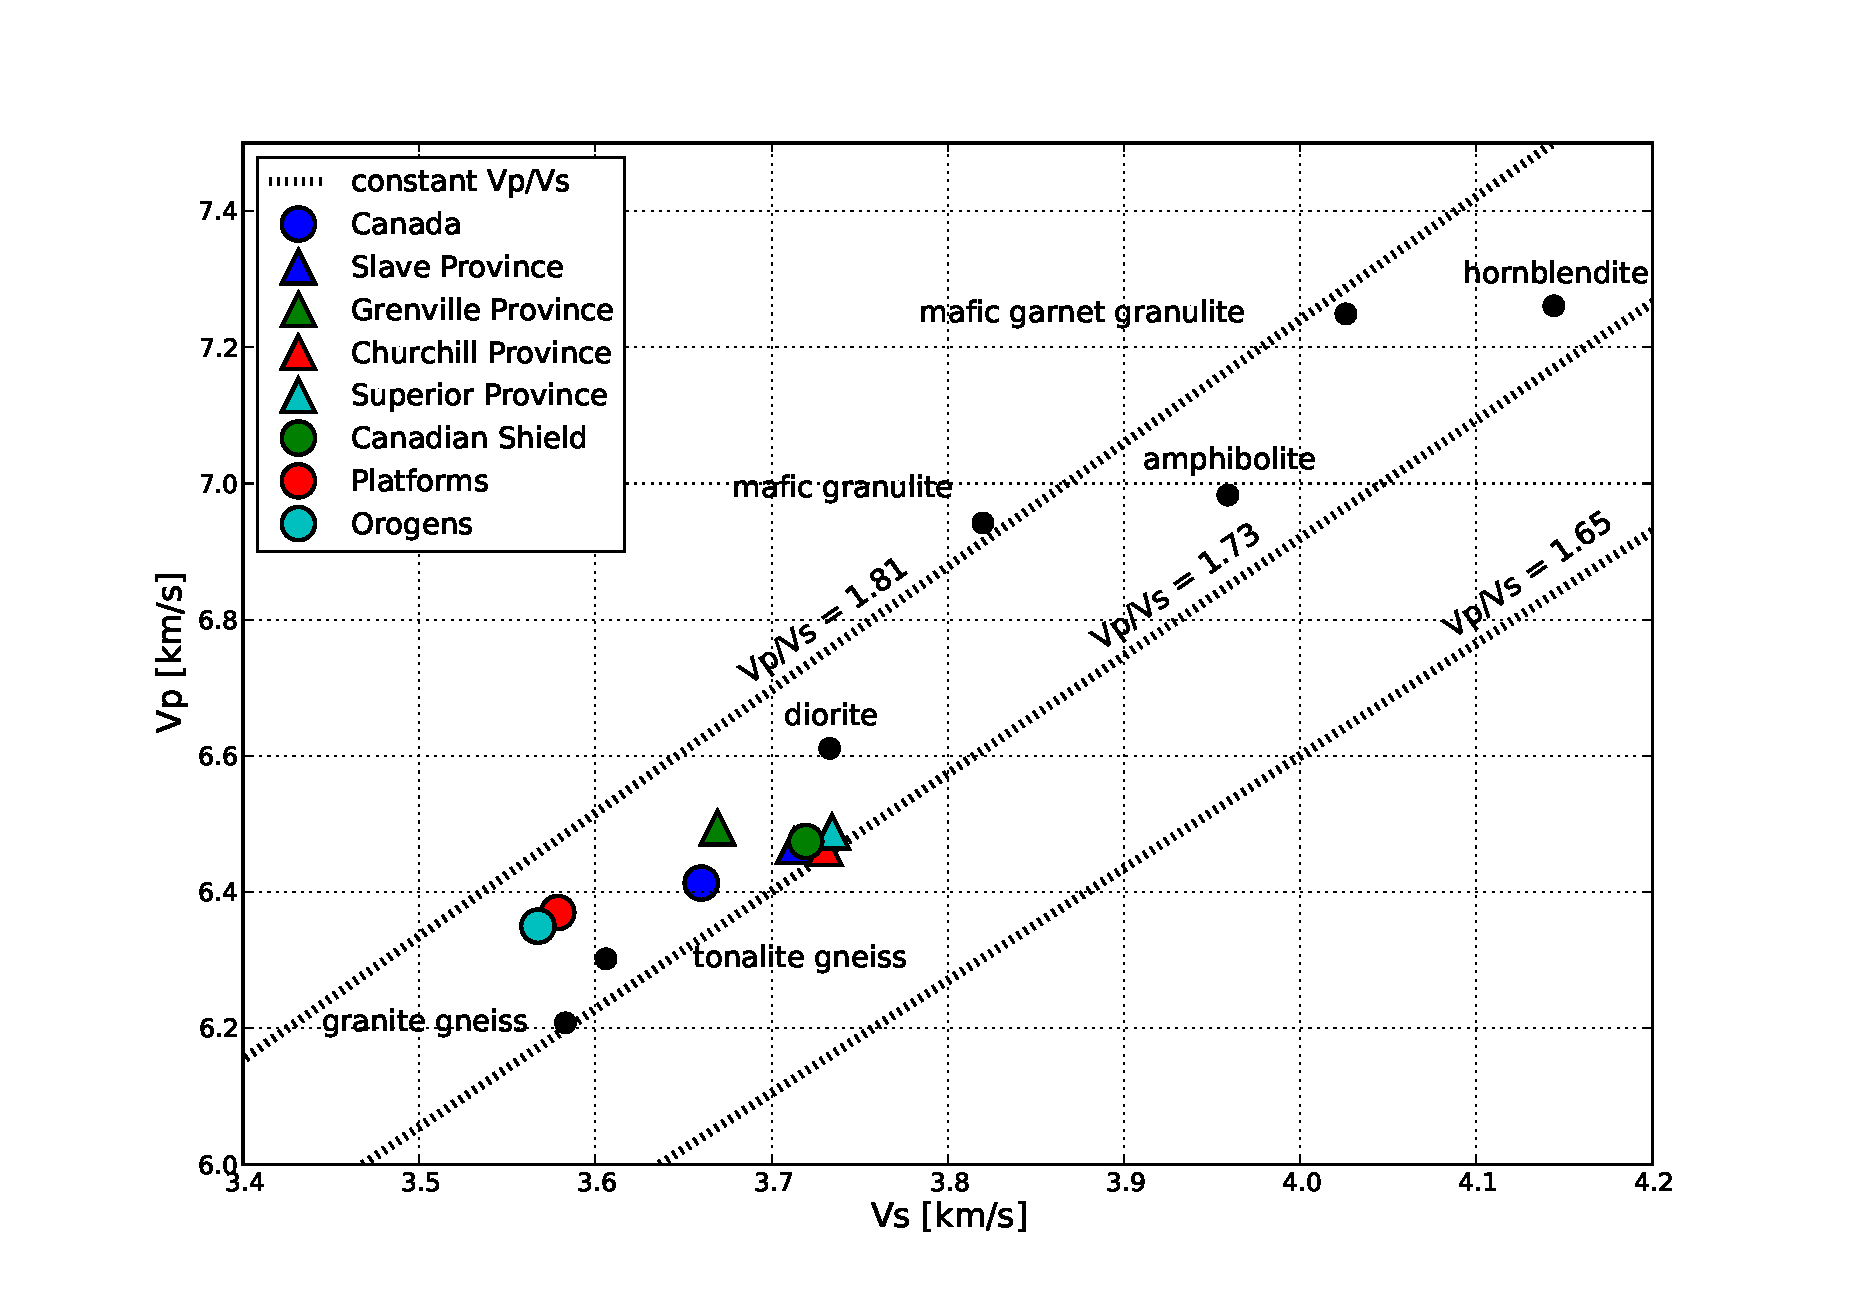
\includegraphics[width=\textwidth]{lithology}
  \caption{$V_P$ and $V_S$ estimates for common crust lithologies and for major Canadian-Shield provinces}
  \label{fig:lith}
\end{figure}


The mean seismic velocity ratio computed in this study is combined with values for $V_P$ from the Crust 1.0 model to enable estimates for $V_P$ and $V_S$ to be used to estimate mean crustal composition. Figure \ref{fig:lith} shows mineral assemblages and weighted Canadian Shield estimates plotted against $V_P$ and $V_S$. Mineral assemblages are chosen as useful representations of common crustal rocks and, specifically, for crust in Shield-like regions. Examples of common shield lithologies can be seen in the 30km of paleo-depth represented in the Kapuskasing uplift in the Superior province [Percival and West, 1994]. This uplift is largely comprised of Archean granite-greenstone terranes dominated by granitoid and gneissic rocks, and contains supracrustal assemblages generally metamorphosed to greenschist to amphibolite facies (hence the inclusion of hornblendite and amphibolite) and early plutonic structures comprised largely of tonalites. Tonalites and granodiorites are also part of the TGG suite (for tonalite-trondhjemite-granodiorite) which dominate Archaean cratons [Rudnick, 1995]. Seismic velocity values for these lithologies are taken from the work of Christensen [1996] and are selected at average crustal pressures of 600 MPa. Lines of constant Poisson's Ratio are plotted for reference.

The Slave, Superior and Churchill provinces share similar mean crustal compositions, with the Slave province being slightly more tonalitic in average composition. These three provinces cluster around the average for the Canadian Shield. The Grenville Province on the other hand differs significantly in mean composition. One interpretation is that the crust in the Grenville province has a mean crustal composition corresponding to a more mafic lower crustal composition than other Shield provinces. This interpretation is consistent with a tectonic model for the the central Grenville Province which suggests that the mid-crust has been completely excised locally [Eaton et. al., 2005; Rivers, 2008]. However, many stations in the South-East of the province also have seismic ratios greater than 1.78, similar to the high values common in the adjacent St. Lawrence Platform (where the geometric mean seismic ratio is 1.79).

 [Any other reasons why Grenville and St. Lawrence Platform have higher R values than rest of Shield???]

[ Continue with crustal composition discussion ]
[ Note: I should include Platforms and Orogens in this paper: will work on this ]

Other researchers have focused on Poisson's Ratio [Zandt and Ammon, 1995] as an indicator of bulk crustal composition as well as crustal thickness [Durrheim and Mooney, 1991] to constrain models of crustal formation. Durrheim and Mooney [1991] compile crustal thickness data and P-wave velocity data for crustal units divided into geochronological ages. They show that Proterozoic crust is thicker than Archean crust and has a higher P-wave velocity. The crustal thickness data attained in this study also show thicker crusts for Proterozoic units (38.9 km) than Archean units (38.0 km) though this difference is not as drastic as the greater than 5km difference reported by Durrheim and Mooney. Though $Vp$ data was not explicity estimated in this study, the higher seismic velocity ratio in the Proterozoic units (1.76) than in Archean units (1.74) aligns with their argument for a thicker basal layer in Proterozoic crustal units.

In contrast, Zandt and Ammon [1995] report high Poisson's Ratio values for Archean Shields and conclude that no systematic difference between Archaean and Proterozoic crust exists. Their average, transformed into $Vp/Vs$, is 1.84, much higher than the wieghted average for the Canadian Shield of 1.74 computed herein. The Authors also report a low $V_P/V_S$ value for Cenozoic-Mesozoic crust, 1.73 compared to the value calculated here of 1.77. Zandt and Ammon interpret these results showing high values for older crust and lower values for younger crust as indicating two end member scenarios. In the uniformitarian model, a delamination type process operates to remove mafic lower crust during continental collisions and is subsequently followed by a stabilizing process involving basaltic underplating. This implies that younger crust has not yet completed the crustal genesis cycle. In their second scenario, Precambrian cratons evolve through unique processes and younger orogens involve recycling and reworking existing material with little crustal growth.

Whereas Zandt and Ammon show increasing $V_P/V_S$ values with crustal age the estimates computed in this study indicate an opposite trend, that is lower seismic velocity ratios with crustal age. This aligns more closely to the results of Durrheim and Mooney [1991] and seems to provide evidence for an evolution of crustal processes throughout geological time. Though Durrheim and Mooney accept the hypothesis that Proterozoic crust is more prone to basaltic underplating, thereby explaining higher velocities and thicker crust, Roberta Rudnick [1995; Rucknick and Gao, 2003] has argued persuasively that a range of possible processes may explain this data.

[ Use crustal composition plus increasing Vp/Vs with younger crust result to make ``best'' pick among the 4 main processes Rudnick proposes to complete section.]




%% -----------------------------------------------%%
\section{Conclusions}

%% ------------------------------------------------------------------------ %%


\section{bibliography}

Bostock, M. G. (1998), Mantle stratigraphy and the evolution of the Slave province, J. Geophys. Res., 103, 21183-21200.

Bostock, M. G., M. R. Kumar (2010), Bias in seismic estimates of crustal properties, J. Geophys. Int., 182, 403-407.

Christensen, N. I. (1996), Poisson's ratio and crustal seismology, J. Geophys. Res., 101, 3139–3156.

Christensen, N. I., W. D. Mooney (1995) Seismic velocity structure and composition of the continental crust: A global view, J. Geophys. Res., 100, 9761-9788.

Darbyshire, F. A., D. W. Eaton, A. W. Frederiksen, E. Leila (2006), New insights into the lithosphere beneath the Superior Province from Rayleigh wave dispersion and receiver function analysis, J. Geophys. Int., 169, 1043-1068.

Durrheim, R. J., W. D. Mooney (1991), Archean and Proterozoic crustal evolution, Geology, 19, 606-609.

Eaton, D. W., S. Dineva, R. Mereu (2005), Crustal thickness and Vp/Vs variations in the Grenville orogen (Ontario, Canada) from analysis of teleseismic receiver functions, Tectonophysics, 420, 223-238.

Efron, B., R. Tibshirani (1986), Bootstrap Methods for Standard Errors, Confidence Intervals, and Other Measures of Statistical Accuracy, Statistical Science, 1, 54-75.

Laske, G., G. Masters, Z. Ma, M. Pasyanos (2013), Update on CRUST1.0 - A 1-degree Global Model of Earth's Crust, Geophys. Res. Abstracts, 15, Abstract EGU2013-2658.

Golub, G. H., M. Heath, G. Wahba (1979), Generalized cross-validation as a method for choosing a good ridge parameter, Technometrics, 21, 215-223.
Mooney, W. D. (2012), Personal communication. Compiled GSC active source data for the Canada.

Kennet, B. L. N., (1991), The removal of free surface interactions from three-component seismograms, J. Geophys. Int., 104, 153-163.

Langston, C. A. (1979), Structure under Mount Rainier, Washington, inferred from teleseismic body waves, J. Geophys. Res., 84(B9), 4749–4762, doi:10.1029/JB084iB09p04749.

Percival, J. A., Gordon F. W. (1994), The Kapuskasing uplift: a geological and geophysical synthesis, Canadian. J. of Earth Sciences, 31, 1256-1286.

Perry, H. K. C., D. W. S. Eaton, A. M. Forte (2002), LITH5.0: a revised crustal model for Canada based on Lithoprobe results,  J. Geophys. Int., 150, 285-294.

Rudnick, R. L. (1995), Making Continental Crust, Nature, 378, 571-578.

Rudnick, R. L., D. M. Fountain (1995), Nature and composition of the continental crust: A lower crustal perspective, Rev. Geophys., 33(3), 267–309, doi:10.1029/95RG01302.

Rudnick, R. L., S. Gao (2003), Composition of the Continental Crust, Treatise on Geochem., 3, 1-64.

Smithson, S. B., R. A. Johnson, Y. K. Wong (1981), Mean crustal velocity: a critical parameter for interpreting crustal structure and crustal growth, Earth and Planetary Science Letters, 53, 323-332.

Taylor, S. R. (1967), The origin and growth of continents, Tectonophysics, 4, 17–34.

Taylor, S. R. (1977), Island arc models and the composition of the continental crust, in Island Arcs, Deep Sea Trenches and Back-Arc Basins, Maurice Ewing Ser., vol. 1, edited by M. Talwani and W. C. Pitman III, pp. 325–335, AGU, Washington, D. C., doi:10.1029/ME001p0325.

Thompson, D. A., I. D. Bastow, G. Helffrich, J.-M. Kendall, J. Wookey, D. B. Snyder, D. W. Eaton (2010), Precambrian crustal evolution: Seismic constraints from the Canadian Shield, Earth and Planetary Science Letters, 297, 655–666.

Zhu, L., H. Kanamori (2000), Moho depth variation in Southern California from teleseismic receiver functions, J. Geophys. Res., 105, 2969-2980.

Zandt, G., C. J. Ammon (1995), Continental crust composition constrained by measurements of crustal Poisson's ratio, Nature, 374, 152-154.




\end{document}

%% ------------------------------------------------------------------------ %%

